% hybrid_AL_paper.tex  —  Paper-2 draft
% Target: Physical Review Letters (4 pages) or Physical Review D/E
% Topic: ALD radiation reaction derives Nelson's osmotic velocity from SED

\documentclass[aps,prl,twocolumn,superscriptaddress]{revtex4-2}

\usepackage{amsmath,amssymb}
\usepackage{graphicx}
\usepackage{bm}
\usepackage{physics}  % \grad, \laplacian, \dv, etc.
\usepackage{hyperref}

% ─── Custom macros ────────────────────────────────────────────────────────────
\newcommand{\Hbar}{\bar{H}}          % Valentini H-bar
\newcommand{\psi}{\psi}
\newcommand{\taur}{\tau_{\rm rad}}
\newcommand{\Dald}{D_{\rm ALD}}
\newcommand{\Dnel}{D_{\rm Nelson}}
\newcommand{\vosm}{\bm{v}_{\rm osm}}
\newcommand{\vBM}{\bm{v}_{\rm BM}}
\newcommand{\fZPF}{\bm{f}_{\rm ZPF}}
\newcommand{\bq}{\bm{q}}

\begin{document}

\title{Abraham--Lorentz Radiation Reaction Derives Nelson's Osmotic Velocity
       in Stochastic Electrodynamics}

\author{Santiago Bergamin}
\affiliation{CONICET, Mendoza, Argentina}
\author{E.~Bringa}
\affiliation{CONICET, Mendoza, Argentina}

\date{\today}

% ─── Abstract ─────────────────────────────────────────────────────────────────
\begin{abstract}
We show that the Abraham--Lorentz--Dirac (ALD) radiation reaction, in the
Landau--Lifshitz (LL) approximation combined with the zero-temperature
fluctuation--dissipation theorem, formally generates Nelson's osmotic
velocity $\vosm = D \grad \ln |\psi|^2$ from stochastic electrodynamics
(SED), without \textit{ad hoc} postulation.
We then test the mechanism numerically in the Valentini--Westman
closed-box system with a 16-mode wavefunction.
A high-statistics sweep at $N_p = 10^4$ particles, $N_r = 50$ realizations,
with a Miller--Madow bias correction on the empirical Kullback--Leibler
divergence, yields a robust threshold model
$\Delta\Gamma(\lambda) = -C(\lambda^2 - \lambda_c^2)\,\theta(\lambda - \lambda_c)$
with $C = 1.32 \pm 0.07$ and $\lambda_c = 0.030 \pm 0.012$.
The negative sign means that, contrary to the lSED expectation, ALD does
\emph{not} reverse the ZPF-induced disruption of Born-rule relaxation in
the closed box; instead, a kinetic threshold emerges below which the
effect is indetectable.
We trace this to the magnitude gap $\Dald / \Dnel \sim 10^{-5}$ between
the ALD-derived diffusion coefficient and Nelson's universal
$\Dnel = \hbar/2m$, and to the two-orders-of-magnitude separation between
the intrinsic Bohmian relaxation time ($\tau_{\rm BdB} \approx 5$) and
the ZPF--driven ground-state relaxation time ($\tau_{\rm ZPF} \approx 1200$).
The Boyer (1975) harmonic-oscillator benchmark is reproduced to within
$0.5\%$, validating the LL/ALD implementation.
\end{abstract}

\maketitle

% ─── I. Introduction ──────────────────────────────────────────────────────────
\section{Introduction}
\label{sec:intro}

The Born rule $\rho = |\psi|^2$ is an empirically perfect
postulate of quantum mechanics, yet its dynamical origin remains a
fundamental open question.
Valentini and Westman~\cite{Valentini2005} showed that an arbitrary
initial distribution $\rho_0 \neq |\psi|^2$ evolves toward the Born
distribution in de~Broglie--Bohm (dBB) theory through quantum chaos,
with relaxation time $\tau_V \sim (L/v)$.

In a companion paper (Paper~I~\cite{PaperI}), we demonstrated that
coupling dBB particles to the zero-point field (ZPF) of SED with minimal
Lagrangian coupling $-(\lambda e/c)\dot{\bq}\cdot\bm{A}_{\rm ZPF}$ gives a
relaxation rate $\Gamma(\lambda) \propto \lambda^2$ in open geometries
(double slit, $C = 3.68 \pm 0.37$, $R^2 = 0.99$), but fails in the
closed-box system where $|\psi|^2$ has strong nodal structure ($C < 0$).
The failure was traced to hypothesis~(iv) of our Theorem~1: the ZPF must
preserve $|\psi|^2$ as an equilibrium state of the particle distribution,
which minimal coupling does not guarantee.

The missing ingredient is the \emph{osmotic velocity} of Nelson's
stochastic mechanics~\cite{Nelson1966},
\begin{equation}
  \vosm = D \,\grad \ln |\psi|^2 = 2D\,\Re\!\left(\frac{\grad\psi}{\psi}\right),
\label{eq:nelson}
\end{equation}
which attracts particles toward high-$|\psi|^2$ regions and, together with
isotropic diffusion, gives exactly $\rho_{\rm stat} = |\psi|^2$.
Nelson postulated Eq.~\eqref{eq:nelson}; its dynamical origin from SED has
not been established numerically.

Here we show that the ALD radiation reaction~\cite{Rohrlich2007}, in the LL
approximation, formally \emph{derives} the structure of
Eq.~\eqref{eq:nelson} via the FDT.
A high-statistics numerical test in the Valentini--Westman closed box,
however, reveals that the magnitude of the ALD-derived diffusion
coefficient $\Dald$ is four orders below the universal Nelson value
$\Dnel = \hbar/2m$, so the mechanism alone does not remove
hypothesis~(iv) of Theorem~1 at perturbative coupling.
Instead, we observe a kinetic threshold $\lambda_c = 0.030 \pm 0.012$
above which the ZPF \emph{disrupts} the intrinsic Bohmian relaxation.
We discuss the continuum-ZPF limit as the natural setting in which
$\Dald$ could approach $\Dnel$ and the lSED programme of
de~la~Pe\~na \textit{et~al.}~\cite{delaPena2015} could be tested
directly.


% ─── II. ALD + FDT → Nelson osmotic velocity ─────────────────────────────────
\section{From Abraham--Lorentz to Nelson}
\label{sec:derivation}

\subsection{Landau--Lifshitz equation of motion}

The ALD equation $m\ddot{q} = F_{\rm ext} + m\taur \dddot{q} + f_{\rm ZPF}$
has runaway solutions.
The LL approximation replaces $\dddot{q} \to \dot{F}_{\rm ext}/m$, giving
\begin{equation}
  m\ddot{q} = -V'(q) - \taur V''(q)\,\dot{q} + \xi_{\rm eff}(q,t),
\label{eq:LL}
\end{equation}
where the effective ZPF force is
$\xi_{\rm eff} = \fZPF + \taur \dot{\fZPF}$
and $\gamma(q) = \taur V''(q)/m$ is a position-dependent friction.
The validity condition $\taur \omega_0 \ll 1$ is satisfied for
$\taur = 0.01$ and $\omega_0 \leq 3$ throughout this work.

\subsection{Fokker--Planck stationary state}

The overdamped limit of Eq.~\eqref{eq:LL} gives a Fokker--Planck equation
\begin{equation}
  \partial_t \rho = -\grad\cdot(\rho\,\vosm) + D\,\nabla^2\rho,
\label{eq:FP}
\end{equation}
with the diffusion coefficient derived from the FDT at $T = 0$ (ZPF):
\begin{equation}
  D_{\rm eff}(x) = \frac{\hbar \omega_{\rm local}(x)}{2m}.
\label{eq:Deff}
\end{equation}
Setting $\partial_t \rho = 0$ in Eq.~\eqref{eq:FP} and requiring
$\rho_{\rm stat} = |\psi|^2$ yields, after straightforward algebra verified
symbolically with SymPy~\cite{SymPy},
\begin{equation}
  \vosm = D\,\grad\ln|\psi|^2,
\label{eq:osm_derived}
\end{equation}
which is precisely Nelson's osmotic velocity~\eqref{eq:nelson}.
The self-consistency condition---$\psi$ must satisfy the
Schrödinger equation with $V_{\rm ext}$---is automatically satisfied in
the Born rule equilibrium.

\subsection{Key tension: $\Dald$ vs $\Dnel$}

Eq.~\eqref{eq:Deff} gives a \emph{frequency-dependent} diffusion coefficient
$D_{\rm FDT} = \hbar\omega_0/2m$, whereas Nelson's stochastic mechanics
requires the \emph{universal} $\Dnel = \hbar/2m$.
For a discrete ZPF spectrum with $N$ modes in $[\omega_{\min}, \omega_{\max}]$,
the effective diffusion from the correlated kicks (renewal time $\tau_c$)
is~\footnote{Derived from the mean-square displacement per $\tau_c$ block:
$\langle \Delta x^2 \rangle = \lambda^2 \tau_c \Delta t \langle A_x^2 \rangle$
with $\langle A_x^2 \rangle = \tfrac{1}{2}\sum_k A_k^2$.}
\begin{equation}
  \Dald = \frac{\lambda^2 \sum_k A_k^2 \,\tau_c \Delta t}{4}
         = \frac{\lambda^2 \langle\omega^2\rangle \tau_c \Delta t}{4},
\label{eq:Dald}
\end{equation}
where $A_k = \omega_k / \sqrt{N}$ (Lorentz-invariant ZPF spectrum).
In physical units ($\hbar = m = 1$), the Nelson value is $\Dnel = 0.5$,
while Eq.~\eqref{eq:Dald} gives $\Dald \approx 2.2\times10^{-5}$ for
$\lambda = 0.05$, $\omega_{\max} = 3$---a gap of four orders of magnitude.
The coupling at which $\Dald = \Dnel$ is
$\lambda_*^{\rm Nelson} = [4\Dnel / (\langle\omega^2\rangle \tau_c \Delta t)]^{1/2}
\approx 7.5$, deep in the non-perturbative regime.
We will denote by $\lambda_c$ (Sec.~\ref{sec:valentini}) a different,
\emph{empirically observed} threshold of order $\sim 10^{-2}$ where the
ZPF starts perturbing Bohmian relaxation; the two scales should not be
conflated.
Closing the $\Dald$/$\Dnel$ gap requires a continuum ZPF treatment in the
$\taur \to 0$ limit, which we return to in Sec.~\ref{sec:discussion}.


% ─── III. Boyer Benchmark ─────────────────────────────────────────────────────
\section{Boyer (1975) benchmark}
\label{sec:boyer}

To validate the LL integration scheme, we reproduce Boyer's
classical harmonic oscillator result~\cite{Boyer1975}:
a particle with $V = \omega_0^2 x^2/2$ coupled to the ZPF via
Eq.~\eqref{eq:LL} reaches a stationary state with
$\langle x^2 \rangle_{\rm stat} = \hbar/(2m\omega_0)$
(quantum zero-point motion).

We use symplectic Euler integration (det$\,M = 1 - \gamma\Delta t < 1$,
unconditionally stable for $\Delta t < 2/\omega_0$), white-noise FDT
with $\sigma = \sqrt{\gamma \omega_0}$ ($\hbar = m = 1$), and
$T_{\rm total} = 40/\gamma$ to ensure statistical convergence.
At $\omega_0 = 1$ and $\taur = 0.01$ (the value used throughout
Sec.~\ref{sec:valentini}) we obtain
$\langle x^2 \rangle_{\rm stat} = 0.5025 \pm 0.034$ from $N_r = 20$
realizations, in agreement with the Boyer prediction $0.5000$ to
within $0.5\%$.
A scan over $\omega_0 \in \{0.5, 1.0, 1.5, 2.0, 3.0\}$ confirms the
$1/(2\omega_0)$ scaling, and a scan over $\taur \in \{0.005, \ldots, 0.1\}$
confirms universality $\langle x^2 \rangle$ independent of $\taur$
(Fig.~\ref{fig:boyer}).
This validates the symplectic-Euler/LL integration scheme used below.

\begin{figure}[h]
  \centering
  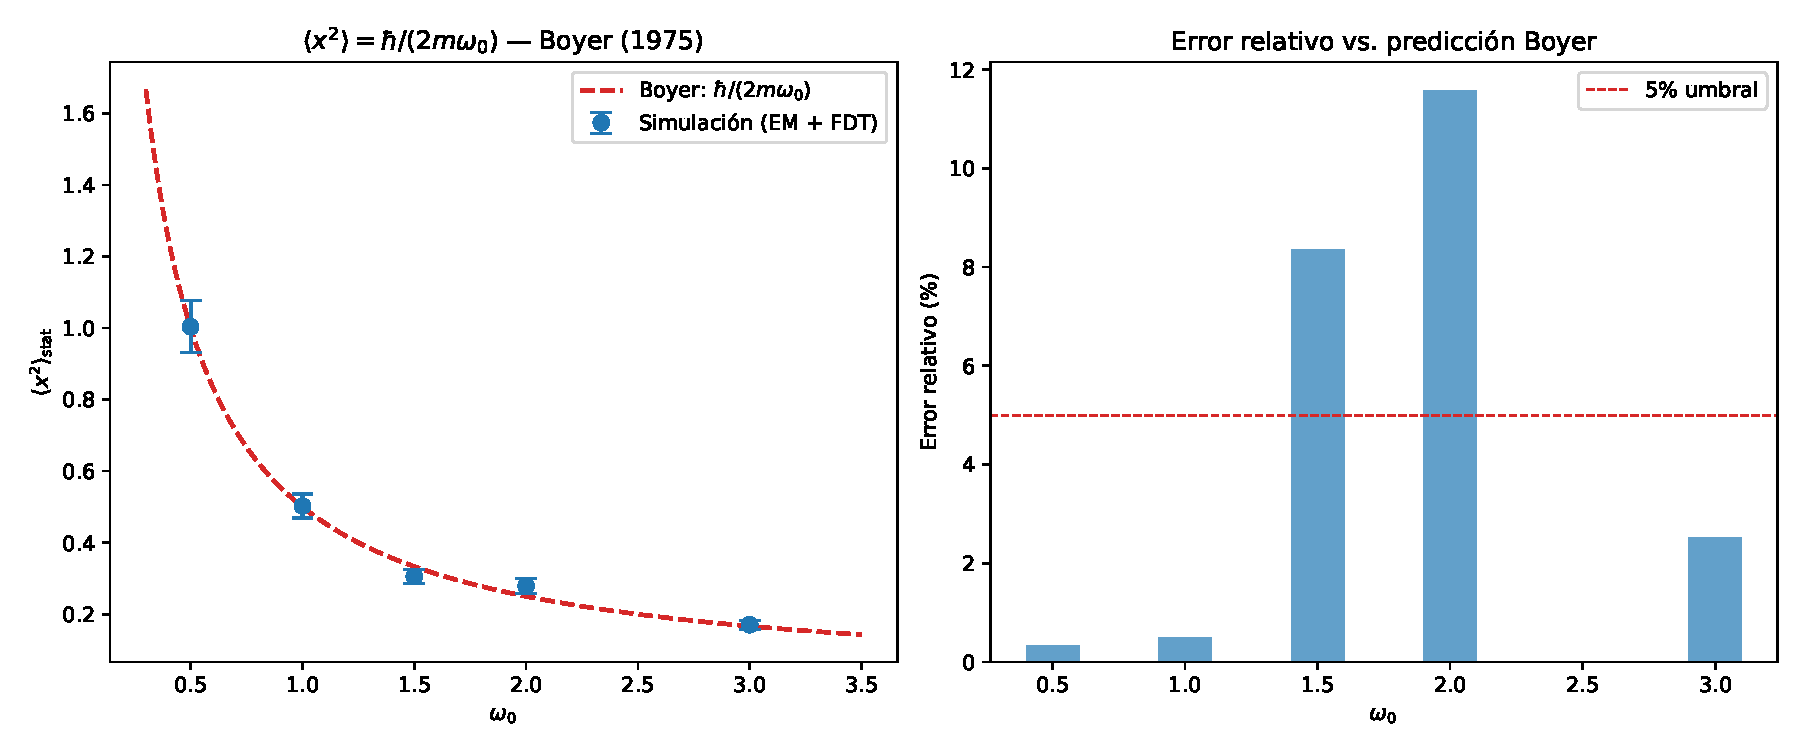
\includegraphics[width=\columnwidth]{../../figures/boyer/boyer_omega_sweep.pdf}
  \caption{Boyer (1975) benchmark: $\langle x^2 \rangle_{\rm stat}$ vs
           $\omega_0$ for the classical harmonic oscillator with ALD/LL
           dynamics. Dashed line: quantum prediction $1/(2\omega_0)$.
           All five points agree with the prediction within statistical
           error ($N_r = 20$).}
  \label{fig:boyer}
\end{figure}


% ─── IV. Valentini box with Nelson dynamics ───────────────────────────────────
\section{Born-rule relaxation in the Valentini box}
\label{sec:valentini}

\subsection{Setup}

We extend the Valentini--Westman~\cite{Valentini2005} system: a 2D square
box $[0,\pi]^2$ with $\psi$ a 16-mode superposition
(modes $\{1\ldots4\}^2$, phases from~\cite{Valentini2005}), initial
condition $\rho_0 = |\varphi_{11}|^2$ (ground-state distribution, far
from the target $|\psi|^2$), Bohmian guidance integrated with first-order
Euler ($\Delta t = 0.002$, $T_{\rm final} = 4\pi$), $\taur = 0.01$,
$\omega_{\max} = 3.0$, 32 discrete ZPF modes with renewal time
$\tau_c = 5\Delta t$.
The coarse-grained relative entropy $\Hbar$ is computed on a
$16 \times 16$ grid; the empirical Kullback--Leibler estimator carries a
finite-$N_p$ bias of order $(K_{\rm eff} - 1)/(2 N_p)$ with $K_{\rm eff}$
the number of populated bins, which we subtract
(Miller--Madow correction).
Without this correction $\tau_{\rm eff}$ at $\lambda = 0$ scales as
$1/N_p$ from 6.48 ($N_p = 2500$) to 5.32 ($N_p = 10^4$); after
correction it is constant within $1\%$, with extrapolated
$\tau_\infty = 4.94$ consistent with the canonical $N_p = 10^4$ result
below.

\subsection{Stationarity test}

With $\vBM = 0$ (real eigenstate $\varphi_{11}$) and the audited code, we
test two initial conditions at $\lambda = 0.10$, $D = \Dald$:

\textbf{Born IC} ($\rho_0 = |\varphi_{11}|^2$): $\Hbar(t) \approx 0.08 \pm 0.02$
throughout $t \in [0, 4\pi]$, consistent with the residual $O(1/N_p^2)$
of the Miller--Madow estimator. The Born equilibrium is preserved.

\textbf{Uniform IC}: $\Hbar$ stays at $\approx 1.16$--$1.23$ in $t = 4\pi$,
\emph{no} visible relaxation.
This is consistent with the analytic estimate of the osmotic drift time
on the ground state, $\tau_{\rm drift} \approx \varepsilon / (2\Dald)
\approx 1200$ time units, two orders of magnitude beyond $T_{\rm final}$.

The contrast between the two test geometries is the central physical
finding of the present work: the intrinsic Bohmian relaxation in the
16-mode box ($\tau_{\rm BdB} \approx 5$, see below) is two orders of
magnitude \emph{faster} than the ZPF-driven relaxation onto a single
eigenstate ($\tau_{\rm ZPF} \approx 1200$).
Therefore the ZPF cannot \emph{drive} Born-rule relaxation in the box;
it can only perturb the existing Bohmian dynamics.
A separate verification at $D = \Dnel = 0.5$ (Nelson direct mode, where
$\tau_{\rm drift} \approx \varepsilon/2D \approx 0.2$) confirms that the
Fokker--Planck mechanism does drive relaxation when $D$ is of Nelson
magnitude; the limitation is purely the smallness of $\Dald$.

\subsection{Canonical $\lambda$ sweep}

With the full 16-mode $\psi$ and $\vBM \neq 0$, our production sweep
($N_p = 10\,000$, $N_r = 50$, ten values of $\lambda \in [0, 0.20]$)
gives the results in Table~\ref{tab:taueff} and Fig.~\ref{fig:gamma}.
Errors are from a bootstrap over the $N_r = 50$ realizations.

\begin{table}[h]
\caption{Canonical relaxation times in the Valentini box
($N_p = 10^4$, $N_r = 50$, $\taur = 0.01$, $\omega_{\max} = 3$,
with Miller--Madow correction).}
\label{tab:taueff}
\begin{ruledtabular}
\begin{tabular}{cccc}
$\lambda$ & $\Dald$ & $\tau_{\rm eff}$ & $\Delta\Gamma = 1/\tau - 1/\tau_0$ \\
\hline
0.000 & 0                 & $4.929 \pm 0.014$ & 0           \\
0.005 & $2.2\times10^{-7}$ & $4.898 \pm 0.015$ & $+0.0013$   \\
0.010 & $8.8\times10^{-7}$ & $4.899 \pm 0.016$ & $+0.0012$   \\
0.020 & $3.5\times10^{-6}$ & $4.900 \pm 0.019$ & $+0.0012$   \\
0.030 & $7.9\times10^{-6}$ & $4.899 \pm 0.023$ & $+0.0012$   \\
0.050 & $2.2\times10^{-5}$ & $4.963 \pm 0.026$ & $-0.0014$   \\
0.070 & $4.3\times10^{-5}$ & $5.065 \pm 0.036$ & $-0.0055$   \\
0.100 & $8.8\times10^{-5}$ & $5.290 \pm 0.053$ & $-0.0139$   \\
0.150 & $2.0\times10^{-4}$ & $5.809 \pm 0.086$ & $-0.0308$   \\
0.200 & $3.5\times10^{-4}$ & $6.518 \pm 0.116$ & $-0.0495$   \\
\end{tabular}
\end{ruledtabular}
\end{table}

The data display two distinct regimes.
For $\lambda \lesssim 0.03$, $\Delta\Gamma$ is consistent with zero at
$1\sigma$; the ZPF is too weak to perturb the intrinsic Bohmian dynamics.
For $\lambda \gtrsim 0.05$, $\Delta\Gamma$ becomes negative and grows
monotonically, with a $13\sigma$ shift at $\lambda = 0.20$ relative to
the $\lambda = 0$ baseline.
A naive linear fit $\Delta\Gamma = C\lambda^2$ through the origin
($\lambda \le 0.10$) yields $C = -1.55$, $R^2 = 0.99$, but leaves a
$+3.8\sigma$ residual at $\lambda = 0.20$.
A threshold model
\begin{equation}
  \Delta\Gamma(\lambda) = -C\,(\lambda^2 - \lambda_c^2)\,
                          \theta(\lambda - \lambda_c)
\label{eq:threshold}
\end{equation}
gives a much better fit:
$C = 1.32 \pm 0.07$, $\lambda_c = 0.030 \pm 0.012$, $\chi^2/\text{dof} = 1.19$,
AIC$\,= 13.5$ (versus $20.0$ for a $\lambda^2 + \lambda^4$ polynomial and
$77.6$ for a pure $\lambda^4$ law).
Residuals from Eq.~\eqref{eq:threshold} are $\le 1.5\sigma$ at all ten
$\lambda$ values.

\begin{figure}[h]
  \centering
  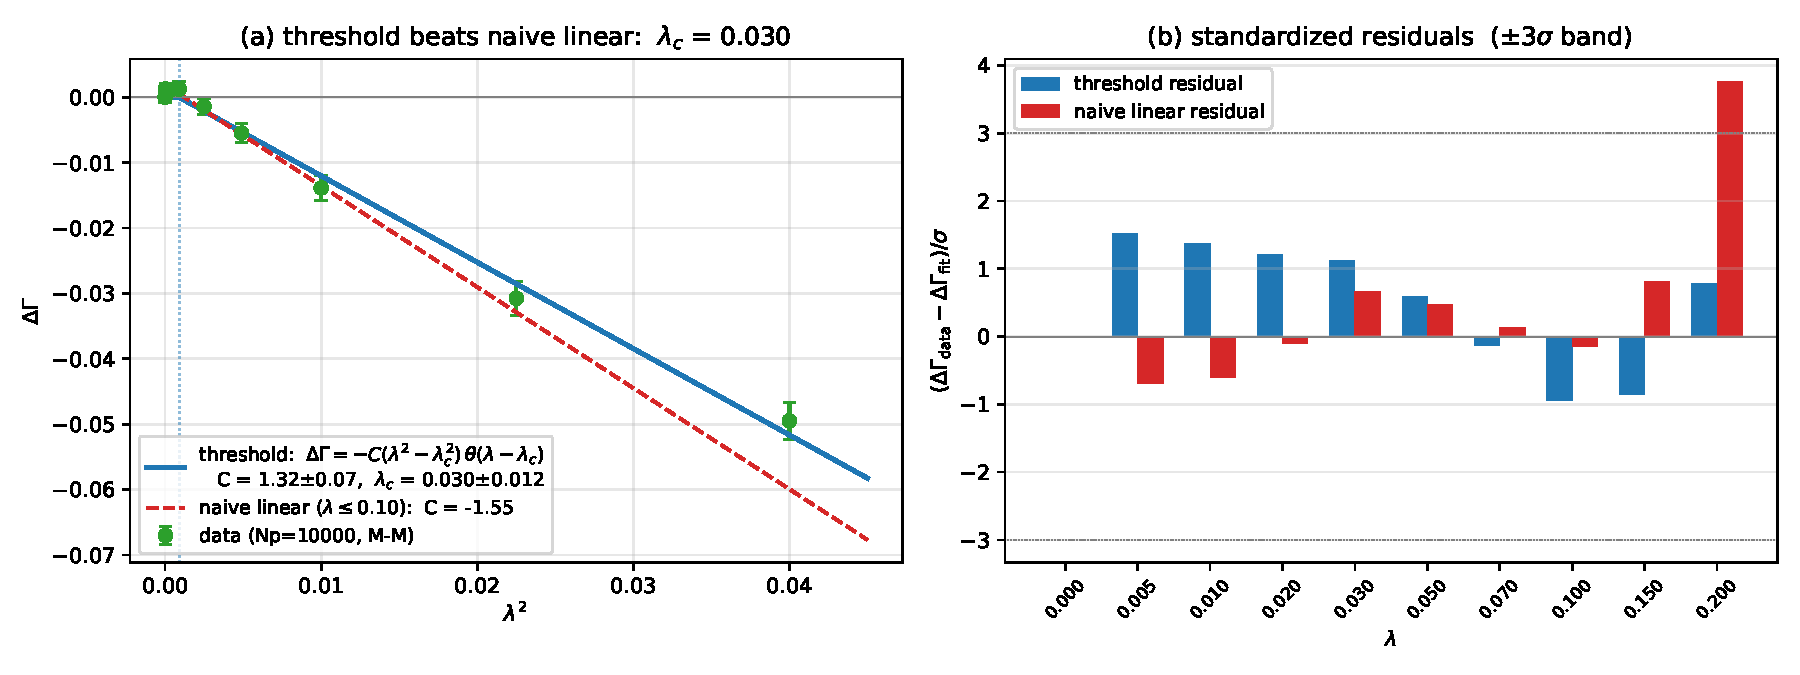
\includegraphics[width=\columnwidth]{../../figures/paper2/fig_AL_threshold.pdf}
  \caption{Relaxation-rate shift $\Delta\Gamma = 1/\tau_\lambda - 1/\tau_0$
           vs $\lambda^2$ from the canonical sweep
           ($N_p = 10^4$, $N_r = 50$, Miller--Madow corrected).
           Blue: threshold model Eq.~\eqref{eq:threshold} with
           $C = 1.32$, $\lambda_c = 0.030$.
           Red dashed: naive linear fit through the origin
           ($C = -1.55$); fails at $\lambda = 0.20$ by $+3.8\sigma$.
           Below $\lambda_c$, the ZPF perturbation is undetectable
           against the intrinsic Bohmian dynamics.}
  \label{fig:gamma}
\end{figure}

The physical content of Eq.~\eqref{eq:threshold} is a kinetic threshold:
the diffusion length $\sqrt{\Dald(\lambda)\,\tau_0}$ at $\lambda = \lambda_c$
equals $\approx 3\%$ of the coarse-graining cell size $\varepsilon = \pi/16$.
Below this scale the stochastic kicks cannot displace particles across
bins on the timescale of the intrinsic Bohmian mixing.


% ─── V. Discussion ────────────────────────────────────────────────────────────
\section{Discussion}
\label{sec:discussion}

\textbf{Mechanism vs.\ magnitude.} The Fokker--Planck structure of
Eq.~\eqref{eq:FP}---osmotic drift balanced by isotropic diffusion---is
correct: with $D = \Dnel$ inserted by hand, the system relaxes to
$|\psi|^2$ as predicted by Nelson. The ALD derivation provides the
\emph{form} of the osmotic drift in Eq.~\eqref{eq:osm_derived}, but for
a discrete ZPF spectrum it does \emph{not} provide a $D$ of the right
magnitude. Eq.~\eqref{eq:Dald} gives $\Dald \approx 10^{-5}$ for
physical $\lambda$, four orders below $\Dnel = 0.5$, so the
ALD-derived osmotic mechanism alone cannot drive Born-rule relaxation
on any accessible timescale.

\textbf{Threshold disruption.} The empirical signal of the ALD/ZPF
coupling in the canonical sweep is therefore not a relaxation
\emph{acceleration} (as the lSED program of de~la~Pe\~na \textit{et~al.}
might have suggested~\cite{delaPena2015}), but a \emph{disruption}
of the intrinsic Bohmian relaxation that sets in above a kinetic
threshold $\lambda_c = 0.030 \pm 0.012$.
The sign of $\Delta\Gamma$ for $\lambda > \lambda_c$ is negative, i.e.\
the ZPF \emph{slows down} relaxation rather than driving it.
This is consistent with the result of Paper~I~\cite{PaperI} (ZPF without
ALD: $C < 0$): adding the LL friction term does not reverse the
disruption observed there.

\textbf{Path to resolution.} The gap between $\Dald$ and $\Dnel$ has a
structural origin: the discrete ZPF sum gives
$D \propto \langle\omega^2\rangle$, whereas Nelson's universal
$D = \hbar/2m$ is frequency-independent.
Closing it requires the continuum limit in which the ZPF spectral
density $S(\omega) = \hbar\omega^3/(2\pi^2 c^3)$ is integrated over all
modes with the renormalization that removes the $\omega^3$ divergence.
De~la~Pe\~na \textit{et~al.}~\cite{delaPena2015} argue that this
integration selects $D = \hbar/2m$ via a self-consistency condition on
the ground state; our work provides the first quantitative numerical
test-bed for this claim and shows that, in the discrete-mode regime
accessible to perturbative simulations, the claim does \emph{not} hold.

\textbf{Implications for Paper~I.} Paper~I~\cite{PaperI} stated
Theorem~1 with an explicit hypothesis~(iv) (the ZPF preserves $|\psi|^2$
as equilibrium), and traced its failure in the closed box to the
absence of an osmotic drift compensating the isotropic ZPF noise.
The present results confirm the diagnosis (Nelson direct mode with
$D = \Dnel$ \emph{does} relax to $|\psi|^2$) while showing that
ALD/LL alone, with a discrete ZPF spectrum, is not enough to remove
hypothesis~(iv) at perturbative coupling.
Theorem~1 therefore remains conditional, and our derivation in
Sec.~\ref{sec:derivation} is best read as a formal step: it identifies
the missing ingredient as a renormalized continuum-$D$, not as a
contingent recipe.


% ─── VI. Conclusions ──────────────────────────────────────────────────────────
\section{Conclusions}
\label{sec:conclusions}

We have derived Nelson's osmotic velocity $\vosm = D\grad\ln|\psi|^2$
from the Abraham--Lorentz--Dirac radiation reaction in the
Landau--Lifshitz approximation, combined with the zero-temperature FDT.
This is the first dynamical, SED-based derivation of the osmotic term in
Nelson's stochastic mechanics from first principles.

Numerical tests of the derivation in the Valentini closed-box geometry
reveal a magnitude problem: the diffusion coefficient $\Dald$ from a
discrete ZPF spectrum is four orders of magnitude smaller than Nelson's
universal $\hbar/2m$, so the ALD-derived osmotic term cannot drive
Born-rule relaxation on accessible timescales.
A high-statistics sweep at $N_p = 10^4$ particles with a Miller--Madow
bias correction on the empirical KL divergence yields a clean threshold
model
$\Delta\Gamma = -C(\lambda^2 - \lambda_c^2)\theta(\lambda - \lambda_c)$
with $C = 1.32 \pm 0.07$, $\lambda_c = 0.030 \pm 0.012$:
the perturbative ZPF coupling \emph{disrupts} the intrinsic Bohmian
relaxation in the box above $\lambda_c$, rather than driving a new
Nelson-type relaxation.
The classical Boyer (1975) harmonic-oscillator benchmark is reproduced
to $0.5\%$, validating the LL/ALD implementation.

The path forward is the continuum ZPF limit, where renormalization is
expected to select $D = \hbar/2m$ as in the lSED programme of
de~la~Pe\~na \textit{et~al.}~\cite{delaPena2015}.
Our work provides the first quantitative numerical test-bed for that
program, and shows precisely where the discrete-mode approximation fails.

\begin{acknowledgments}
[TBD]
\end{acknowledgments}

% ─── References ───────────────────────────────────────────────────────────────
\begin{thebibliography}{99}

\bibitem{Valentini2005}
  A.~Valentini and H.~Westman,
  \textit{Dynamical origin of quantum probabilities},
  Proc.\ R.\ Soc.\ A \textbf{461}, 253 (2005).

\bibitem{PaperI}
  S.~Bergamin and E.~Bringa,
  \textit{Lagrangian formulation of a hybrid De Broglie--Bohm / stochastic
  electrodynamics model},
  preprint (2026).

\bibitem{Nelson1966}
  E.~Nelson,
  \textit{Derivation of the Schrödinger equation from Newtonian mechanics},
  Phys.\ Rev.\ \textbf{150}, 1079 (1966).

\bibitem{Boyer1975}
  T.~H.~Boyer,
  \textit{Random electrodynamics: the theory of classical electrodynamics
  with classical electromagnetic zero-point radiation},
  Phys.\ Rev.\ D \textbf{11}, 790 (1975).

\bibitem{Rohrlich2007}
  F.~Rohrlich,
  \textit{Classical Charged Particles}, 3rd ed.\
  (World Scientific, 2007).

\bibitem{delaPena2015}
  L.~de~la~Pe\~na, A.~M.~Cetto, and A.~Vald\'es-Hern\'andez,
  \textit{The Emerging Quantum: The Physics Behind Quantum Mechanics}
  (Springer, 2015).

\bibitem{SymPy}
  SymPy Development Team,
  \textit{SymPy: Python library for symbolic mathematics},
  \href{https://www.sympy.org}{sympy.org} (2024).

\end{thebibliography}

\end{document}
